\begin{center}
	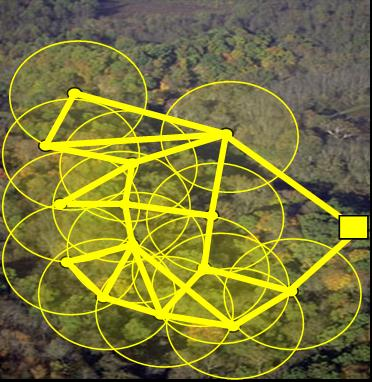
\includegraphics{img/env.jpg}
\end{center}

Wireless sensor network are deployed in a wide range of environments. This affects
the away the routing protocols perform and the way hierarchies are formed. An indoor
environment for example means that the nodes will have to use more power to transmit
packets which will lead to lower battery life. We think it is important to be able to
see how this protocols behave in a real environment. This will be very important for
mobile nodes, which can change their location, as simple attenuation based design will
not be able to simulate realistically the effects of the environment on power needed to
transmit.

The environment will not be limited to the topology of the environment but will also 
include:
\begin{itemize}
	\item Nodes. For simulating nodes placed in a fixed way(useful when running the same
simulation more than once) the nodes can be placed directly in the environment.
	\item Data sources. To simulate data for the networks, data sources will be placed in
the environment, when a node gets in contact with it, the sensor will generate data packets. 
They can be stationary, mobile or affect an area.
\end{itemize}

Environments will be designed in Blender, a 3D graphics tool, from which they will be
exported to our simulator using its extensive scripting support. They will be visible
in the gui of \codename, along with the nodes.


